\documentclass{beamer}

\usepackage{algorithm}
\usepackage{algpseudocode}

\usefonttheme{serif}
\usepackage{dsfont}
\setbeamersize{text margin left=5pt, text margin right=5pt}

\newcommand{\bgk}[1]{\boldsymbol{#1}}

\newcommand{\bzero}{\bgk{0}}
\newcommand{\bone}{\bgk{1}}

\newcommand{\balpha}{\bgk{\alpha}}
\newcommand{\bnu}{\bgk{\nu}}
\newcommand{\bbeta}{\bgk{\beta}}
\newcommand{\bxi}{\bgk{\xi}}
\newcommand{\bgamma}{\bgk{\gamma}} 
\newcommand{\bo}{\bgk{o }}
\newcommand{\bdelta}{\bgk{\delta}}
\newcommand{\bpi}{\bgk{\pi}}
\newcommand{\bepsilon}{\bgk{\epsilon}} 
\newcommand{\bvarepsilon}{\bgk{\varepsilon}} 
\newcommand{\brho}{\bgk{\rho}}
\newcommand{\bvarrho}{\bgk{\varrho}}
\newcommand{\bzeta}{\bgk{\zeta}}
\newcommand{\bsigma}{\bgk{\sigma}}
\newcommand{\boldeta}{\bgk{\eta}}
\newcommand{\btay}{\bgk{\tau}}
\newcommand{\btheta}{\bgk{\theta}}
\newcommand{\bvertheta}{\bgk{\vartheta}}
\newcommand{\bupsilon}{\bgk{\upsilon}}
\newcommand{\biota}{\bgk{\iota}}
\newcommand{\bphi}{\bgk{\phi}}
\newcommand{\bvarphi}{\bgk{\varphi}}
\newcommand{\bkappa}{\bgk{\kappa}}
\newcommand{\bchi}{\bgk{\chi}}
\newcommand{\blambda}{\bgk{\lambda}}
\newcommand{\bpsi}{\bgk{\psi}}
\newcommand{\bmu}{\bgk{\mu}}
\newcommand{\bomega}{\bgk{\omega}}

\newcommand{\bA}{\bgk{A}}
\newcommand{\bDelta}{\bgk{\Delta}}
\newcommand{\bLambda}{\bgk{\Lambda}}
\newcommand{\bSigma}{\bgk{\Sigma}}
\newcommand{\bOmega}{\bgk{\Omega}}

\newcommand{\bvec}[1]{\mathbf{#1}}

\newcommand{\va}{\bvec{a}}
\newcommand{\vb}{\bvec{b}}
\newcommand{\vc}{\bvec{c}}
\newcommand{\vd}{\bvec{d}}
\newcommand{\ve}{\bvec{e}}
\newcommand{\vf}{\bvec{f}}
\newcommand{\vg}{\bvec{g}}
\newcommand{\vh}{\bvec{h}}
\newcommand{\vi}{\bvec{i}}
\newcommand{\vj}{\bvec{j}}
\newcommand{\vk}{\bvec{k}}
\newcommand{\vl}{\bvec{l}}
\newcommand{\vm}{\bvec{m}}
\newcommand{\vn}{\bvec{n}}
\newcommand{\vo}{\bvec{o}}
\newcommand{\vp}{\bvec{p}}
\newcommand{\vq}{\bvec{q}}
\newcommand{\vr}{\bvec{r}}
\newcommand{\vs}{\bvec{s}}
\newcommand{\vt}{\bvec{t}}
\newcommand{\vu}{\bvec{u}}
\newcommand{\vv}{\bvec{v}}
\newcommand{\vw}{\bvec{w}}
\newcommand{\vx}{\bvec{x}}
\newcommand{\vy}{\bvec{y}}
\newcommand{\vz}{\bvec{z}}

\newcommand{\vA}{\bvec{A}}
\newcommand{\vB}{\bvec{B}}
\newcommand{\vC}{\bvec{C}}
\newcommand{\vD}{\bvec{D}}
\newcommand{\vE}{\bvec{E}}
\newcommand{\vF}{\bvec{F}}
\newcommand{\vG}{\bvec{G}}
\newcommand{\vH}{\bvec{H}}
\newcommand{\vI}{\bvec{I}}
\newcommand{\vJ}{\bvec{J}}
\newcommand{\vK}{\bvec{K}}
\newcommand{\vL}{\bvec{L}}
\newcommand{\vM}{\bvec{M}}
\newcommand{\vN}{\bvec{N}}
\newcommand{\vO}{\bvec{O}}
\newcommand{\vP}{\bvec{P}}
\newcommand{\vQ}{\bvec{Q}}
\newcommand{\vR}{\bvec{R}}
\newcommand{\vS}{\bvec{S}}
\newcommand{\vT}{\bvec{T}}
\newcommand{\vU}{\bvec{U}}
\newcommand{\vV}{\bvec{V}}
\newcommand{\vW}{\bvec{W}}
\newcommand{\vX}{\bvec{X}}
\newcommand{\vY}{\bvec{Y}}
\newcommand{\vZ}{\bvec{Z}}

\usepackage{subcaption}
\newcommand{\bitem}{\item[$\bullet$]}

\usepackage{xcolor}
\usepackage[utf8]{inputenc}
\DeclareFontEncoding{LS1}{}{}
\DeclareFontSubstitution{LS1}{stix}{m}{n}
\DeclareSymbolFont{symbols2}{LS1}{stixfrak} {m} {n}
\DeclareMathSymbol{\operp}{\mathbin}{symbols2}{"A8}
\setbeamertemplate{navigation symbols}{}

\usepackage{lipsum}

\newcommand\blfootnote[1]{%
  \begingroup
  \renewcommand\thefootnote{}\footnote{#1}%
  \addtocounter{footnote}{-1}%
  \endgroup
}

\addtobeamertemplate{navigation symbols}{}{%
    \usebeamerfont{footline}%
    \usebeamercolor[fg]{footline}%
    \hspace{1em}%
    \insertframenumber/\inserttotalframenumber
}

\title{
Sketching\\
Lecture 8
}
%\subtitle{Mathematical framework, existence and exactness}

\author{F. M. Faulstich}
\date{02/02/2024}


\begin{document}

\frame{\titlepage}

\begin{frame}{What is sketching?}

It is a dimension reduction:\\
\begin{itemize}
    \bitem Let $\vA \in \mathbb{F}^{n \times m}$. \\
    A matrix $\vS\in \mathbb{F}^{d \times n}$ with $d \ll n$ is called a sketching matrix. We sketch $\vA$ by applying $\vS \vA$
    \only<1>{
    \begin{figure}
        \centering
        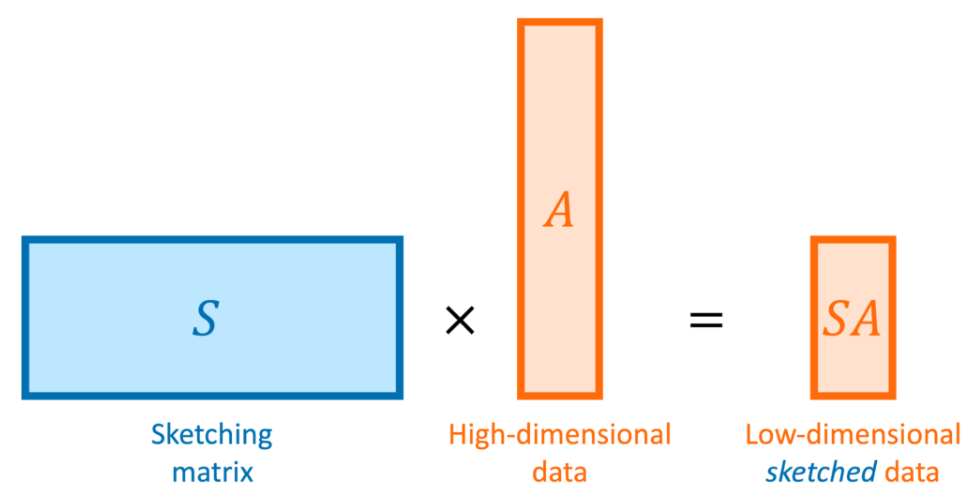
\includegraphics[width = 0.5\textwidth]{Graphics/Sketching.png}
    \end{figure}
    }
    \pause
    \bitem Consider $\vA = [\va_n|...|\va_m]$. The matrix $\vS$ is a good sketch if
    $$
    (1-\varepsilon) \Vert \va_i \Vert
    \leq 
    \Vert \vS \va_i \Vert
    \leq 
    (1+\varepsilon) \Vert \va_i \Vert
    $$
    the lengths of the vectors are preserved.\\
    (Distortion condition)
    \bitem In linear algebra, we want to sketch
    $$
    {\rm Im}(\vA) = \{\vA\vx ~|~ \vx \in\mathbb{F}^{m} \}
    $$
    \bitem There exists sketching matrices that achieve $\varepsilon$ distortion for ${\rm Im}(\vA)$ with an output dimension
    $$
    d \approx m/\varepsilon^2
    $$
\end{itemize}
    
\end{frame}


\begin{frame}{Sketching matrices}

\begin{center}
    Sketching is {\bf not} unique!
\end{center}
    
\end{frame}

\begin{frame}{Sketching matrices}

\begin{itemize}
    \bitem  Random projections\\
    \bitem Johnson-Lindenstrauss lemma:\\
    Given $0<\varepsilon <1$, a set $X$ of $m\in \mathbb {Z} _{\geq 1}$ points in $\mathbb {R} ^{N}$ ($N\in \mathbb {Z} _{\geq 0}$), and an integer $n>8(\ln m)/\varepsilon ^{2}$, there exists a linear map $f:\mathbb {R} ^{N}\rightarrow \mathbb {R} ^{n}$ such that
    $$
    (1-\varepsilon )\|u-v\|^{2}\leq \|f(u)-f(v)\|^{2}\leq (1+\varepsilon )\|u-v\|^{2}
    $$
    for all $ u,v\in X$.\\~\\
    \begin{center}
    ``a small set of points in high-dimensional space can be embedded into a lower-dimensional space in such a way that the distances between the points are nearly preserved.''
    \end{center}
\end{itemize}
    
\end{frame}


\begin{frame}{Gaussian Embeddings}

\begin{itemize}
    \bitem $\mathbb{F}^{d \times n} \ni \vS\sim \mathcal{N}(\bzero, \frac{1}{d}\vI)$, i.e., the entries of $\vS$ are i.i.d.~$\mathcal{N}(0,\frac{1}{d})$
    \bitem Sketches ${\rm Im}(\vA)$ well\\
    \bitem Benefits:\\
    Easy to code\\
    Requires only the standard matrix product\\
    choose $d \approx m/\varepsilon^2$
    \bitem Downsides:\\
    Sketching a vector $\va\in\mathbb{F}^{n}$ costs $\mathcal{O}(dn)$\\
    Additional storage required for $\vS$
\end{itemize}

\end{frame}

\begin{frame}{{\small Subsampled Randomized Trigonometric Transforms (SRTT)}}

\begin{itemize}
    \bitem Ansatz
    $$
    \vS 
    =
    \sqrt{\frac{n}{d}} \vR \vF \vD
    $$
    where: 
    \begin{itemize}
        \item $\vD \in \mathbb{F}^{n \times n}$ diagonal with Rademacher i.i.d.~entries \hfill $[\mathcal{O}(n)]$
        \item $\vF \in \mathbb{F}^{n \times n}$ fast trigonometric transform\\
         e.g. discrete cosine transform
        \item $\vR \in \mathbb{F}^{d \times n}$ is a selection matrix.  \hfill $[\mathcal{O}(d)]$\\
        Let $\{i_1,...,i_d\}\subset [\![n [\!]$, then $\vR \vb := (b_{i_1},...,b_{i_d})$ 
    \end{itemize}
    \bitem Benefits:\\
    Sketching a vector $\va\in\mathbb{F}^{n}$ costs $\mathcal{O}(n {\rm log}(n))$
    \bitem Drawbacks:\\
    SRTT requires a good implementation of a fast trigonometric transform.\\
    choose $d \approx (m {\rm log}(m))/\varepsilon^2$    
\end{itemize}
    
\end{frame}


\begin{frame}{Discrete cosine transform (DCT)}
\begin{itemize}
    \bitem Similar to discrete Fourier transform but real valued coefficients 
    \bitem DCT--II: Let $\vx\in\mathbb{R}^n$
    $$
    \vy_k = \sum_{i=0}^{n-1} \vx_{i} \cos \left(\frac{\pi}{n}\left(i+\frac{1}{2}\right)k \right)
    \qquad {\rm for ~} k=0,...,n-1
    $$
    \bitem Can be implemented fast! $\mathcal{O} (n \log(n))$
\end{itemize}
    
\end{frame}


\begin{frame}{SRTT (MATLAB)}

\begin{figure}
    \centering
    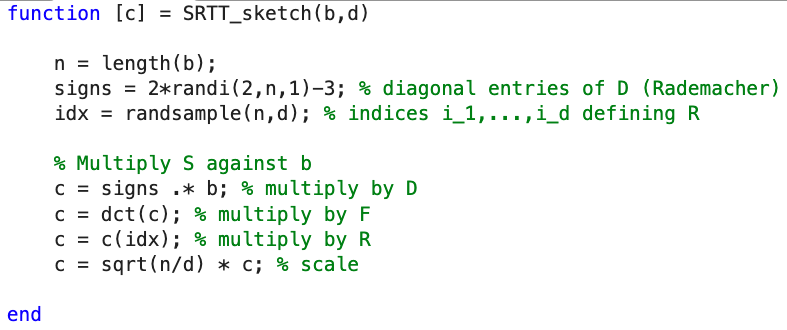
\includegraphics[width = 0.8\textwidth]{Graphics/SRTT.png}
\end{figure}
    
\end{frame}


\begin{frame}{Sparse Sign Embeddings (SSE)}

\begin{itemize}
    \bitem Ansatz
    $$
    \vS = \frac{1}{\sqrt{\zeta}} [\vs_1|...|\vs_n]
    $$
    $\vs_i\in\mathbb{F}^d$ are random vectors with $\mathbb{N} \ni \zeta$ many Rademacher entries.\\
    In practice, $\zeta$ is small like $8$.
    \bitem Benefits:\\
    Using a sparse library $\vS$ can applied super fast! $ \mathcal{O}(n)$ or $\mathcal{O}(n {\rm log(d)})$\\
    \begin{center}
        With a good sparse matrix library, sparse sign embeddings are often the fastest sketching matrix by a wide margin
    \end{center}
    \bitem Drawbacks:\\
    Larger storage than SRTT: $\mathcal{O}(\zeta n)$ vs $\mathcal{O}(n)$
\end{itemize}
\end{frame}


\begin{frame}{Comparison (time)}

We compare:
\begin{itemize}
    \bitem Construction: The time required to generate the sketching matrix $\vS$.
    \bitem Vector apply. The time to apply the sketch to a single vector
    \bitem Matrix apply. The time to apply the sketch to an $n\times 200$ matrix
\end{itemize}

Settings and parameters:
\begin{itemize}
    \bitem We will test with input dimension $n = 10^6$ and $d = 400$.
    \bitem We use SRTT with DCT
    \bitem We use $\zeta = 8$ for SSE
\end{itemize}
    
\end{frame}

\begin{frame}{Comparison (time)}

Averaged times over 20 runs:

    \begin{figure}
        \centering
        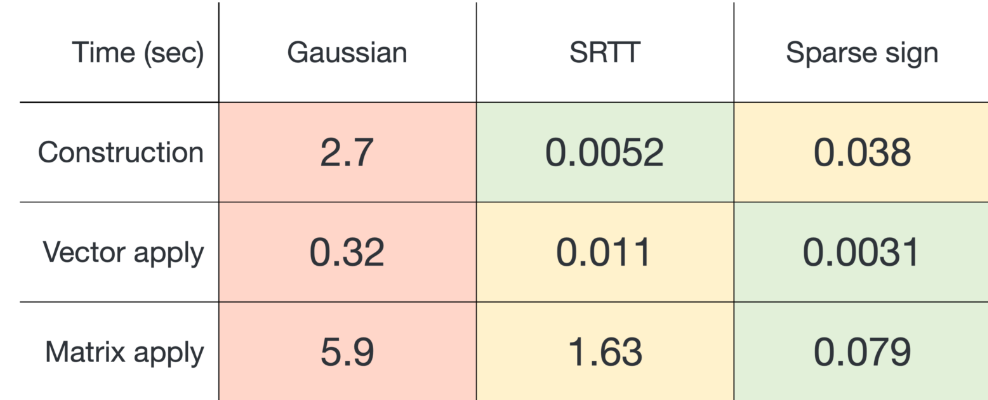
\includegraphics[width = 0.8\textwidth]{Graphics/Timings.png}
    \end{figure}

Conclusion:\\
\begin{itemize}
    \bitem SSE are the fastest sketching matrices by a wide margin! 
    \bitem For an ``end-to-end'' workflow involving generating the sketching matrix $\vS \in \mathbb{R}^{400\times 10^6}$ and applying it to a matrix $\vA\in\mathbb{R}^{10^6\times 200}$, SSE are 14x faster than SRTTs and 73x faster than Gaussian embeddings. 
\end{itemize}
    
\end{frame}

\begin{frame}{How to use sketching?}

Sketch-and-solve:
\begin{itemize}
    \bitem Apply sketch to perform a dimension reduction
    \bitem Apply conventional numerical linear algebra tools
\end{itemize}
~\\
Example: Least-squares problem
$$
\min_{\vx \in \mathbb{R}^{m}} \Vert \vA \vx - \vb \Vert
$$
\begin{itemize}
    \bitem What do we sketch? 
    \bitem We sketch: $\vA$ and $\vb$
    \bitem Then solve
    $$
    \min_{\hat \vx \in \mathbb{R}^{m}} \Vert (\vS\vA) \hat\vx - \hat \vb \Vert
    $$
\end{itemize}

\end{frame}

\begin{frame}{Does this work?}

\begin{itemize}
    \bitem Let $\vx_*$ be the solution to 
    $$
    \min_{\vx \in \mathbb{R}^{m}} \Vert \vA \vx - \vb \Vert
    $$
    and let $\hat \vx$ be the sketch-and-solve solution
    \bitem Using the distortion condition we get
    $$
    \Vert \vA \hat \vx - \vb\Vert
    \leq 
    \frac{1+\varepsilon}{1-\varepsilon} \Vert \vA \vx - \vb\Vert
    $$
    \bitem for $\varepsilon = 1/3$ this yields
    $$
    \Vert \vA \hat \vx - \vb\Vert
    \leq 
    2 \Vert \vA \vx_* - \vb\Vert
    $$
\end{itemize}

\begin{center}
    $\Rightarrow$ Good? Bad?
\end{center}

\end{frame}


\begin{frame}{Numerics}

Experiment:
~\\
\begin{itemize}
    \bitem Consider a least-squares problem of size 10,000 by 100 with condition number $10^8$ and residual norm $10^{-4}$
    \bitem Generate SSE $d = 400$ with $\varepsilon \approx 1/2$
\end{itemize}
~\\
Findings:
\begin{itemize}
    \bitem Rsidual norms:
    \begin{itemize}
        \item sketch-and-solve: 1.13e-4
        \item direct: 1.00e-4
    \end{itemize} 
    \bitem Forward errors:
        \begin{itemize}
        \item sketch-and-solve: 1.06e+3
        \item direct: 8.08e-7
    \end{itemize} 
\end{itemize}
~\\
Conclusion:
\begin{center}
    If a small enough residual is all that is needed, then sketch-and-solve is perfectly adequate.
    If a small forward error is needed, sketch-and-solve can be quite bad.
\end{center}

\end{frame}

\begin{frame}{Can we do better?}

\begin{itemize}
    \bitem Sketch-and-solve is a fast way to get a low-accuracy solution to a least-squares problem 
    \bitem How about iterative methods?
    \bitem Observer that 
    $$
    \vS \vA = \vQ \vR 
    \Rightarrow
    \vA^\top \vA
    \approx 
    (\vS \vA)^\top (\vS \vA)
    =
    \vR^\top \vQ^\top  \vQ \vR
    =
    \vR^\top \vR
    $$
    \bitem Using normal equations we can then solve the LSP iteratively
    \begin{itemize}
        \item[i)] Solving
        $$
        (\vA^\top \vA) \vx = \vA^\top \vb 
        \Rightarrow 
        \vx \approx \vx_1 = \vR^{-1} \vR^{-\top} \vA^\top \vb 
        $$
        \item[ii)] Solve for the resiudal
        $$
        \vA^\top \vA (\vx - \vx_0)
        =
        \vA^\top (\vb - \vA \vx_0)
        \Rightarrow
        \vx \approx 
        \vx_2
        =
        \vx_1 + \vR^{-1} \vR^{-\top}\vA^\top (\vb - \vA \vx_1) 
        $$
        $\vdots$
        \item[n)] $\vx_n
        =
        \vx_{n-1} + \vR^{-1} \vR^{-\top}\vA^\top (\vb - \vA \vx_{n-1})$
    \end{itemize}
\end{itemize}

\begin{center}
    $\Rightarrow$ Iterative sketching
\end{center}
\end{frame}

\begin{frame}{Comparison}

\begin{figure}
    \centering
    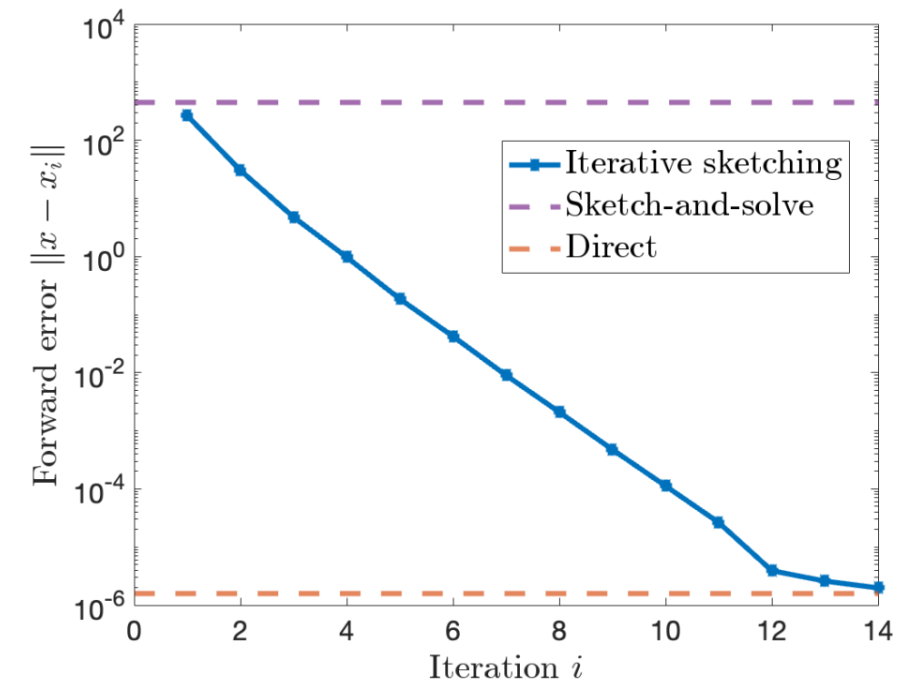
\includegraphics[width = 0.6\textwidth]{Graphics/IterativeSketching.png}
\end{figure}


\end{frame}

\end{document}




